\documentclass[conference]{IEEEtran}
%\IEEEoverridecommandlockouts
% The preceding line is only needed to identify funding in the first footnote. If that is unneeded, please comment it out.
\usepackage{cite}
\usepackage{amsmath,amssymb,amsfonts}
\usepackage{algorithmic}
\usepackage[bottom]{footmisc}
\usepackage{graphicx}
\usepackage{textcomp}
\usepackage{xcolor}
\def\BibTeX{{\rm B\kern-.05em{\sc i\kern-.025em b}\kern-.08em
    T\kern-.1667em\lower.7ex\hbox{E}\kern-.125emX}}
\begin{document}

\title{Internet Routing Security}

\maketitle

\section{Introduction}
Imagine you are listening to a playlist on Youtube and the music suddenly stops.  It seems like you still have access to other websites, so this must be a technical problem at Youtube, right?  Back in 2008, something similar happened to people across the globe, but it had nothing to do with technical issues at Youtube.  Instead, the state run network of Pakistan caused all Youtube traffic to be diverted into the network equivalent of a black hole.  It turned out that Pakistan was simply trying to block Youtube for users within its borders, and yet it still managed to take Youtube down for almost all users across the world.  How could a network in Pakistan cause users in Boston to be unable to reach services hosted in California?  And if this is possible, couldn't this same technique be used by cyber criminals to steal sensitive information?  In this section, we will address how this is possible and what can be done to mitigate it.

\section{Internet Routing: Address and Number Assignment}
\begin{figure}
  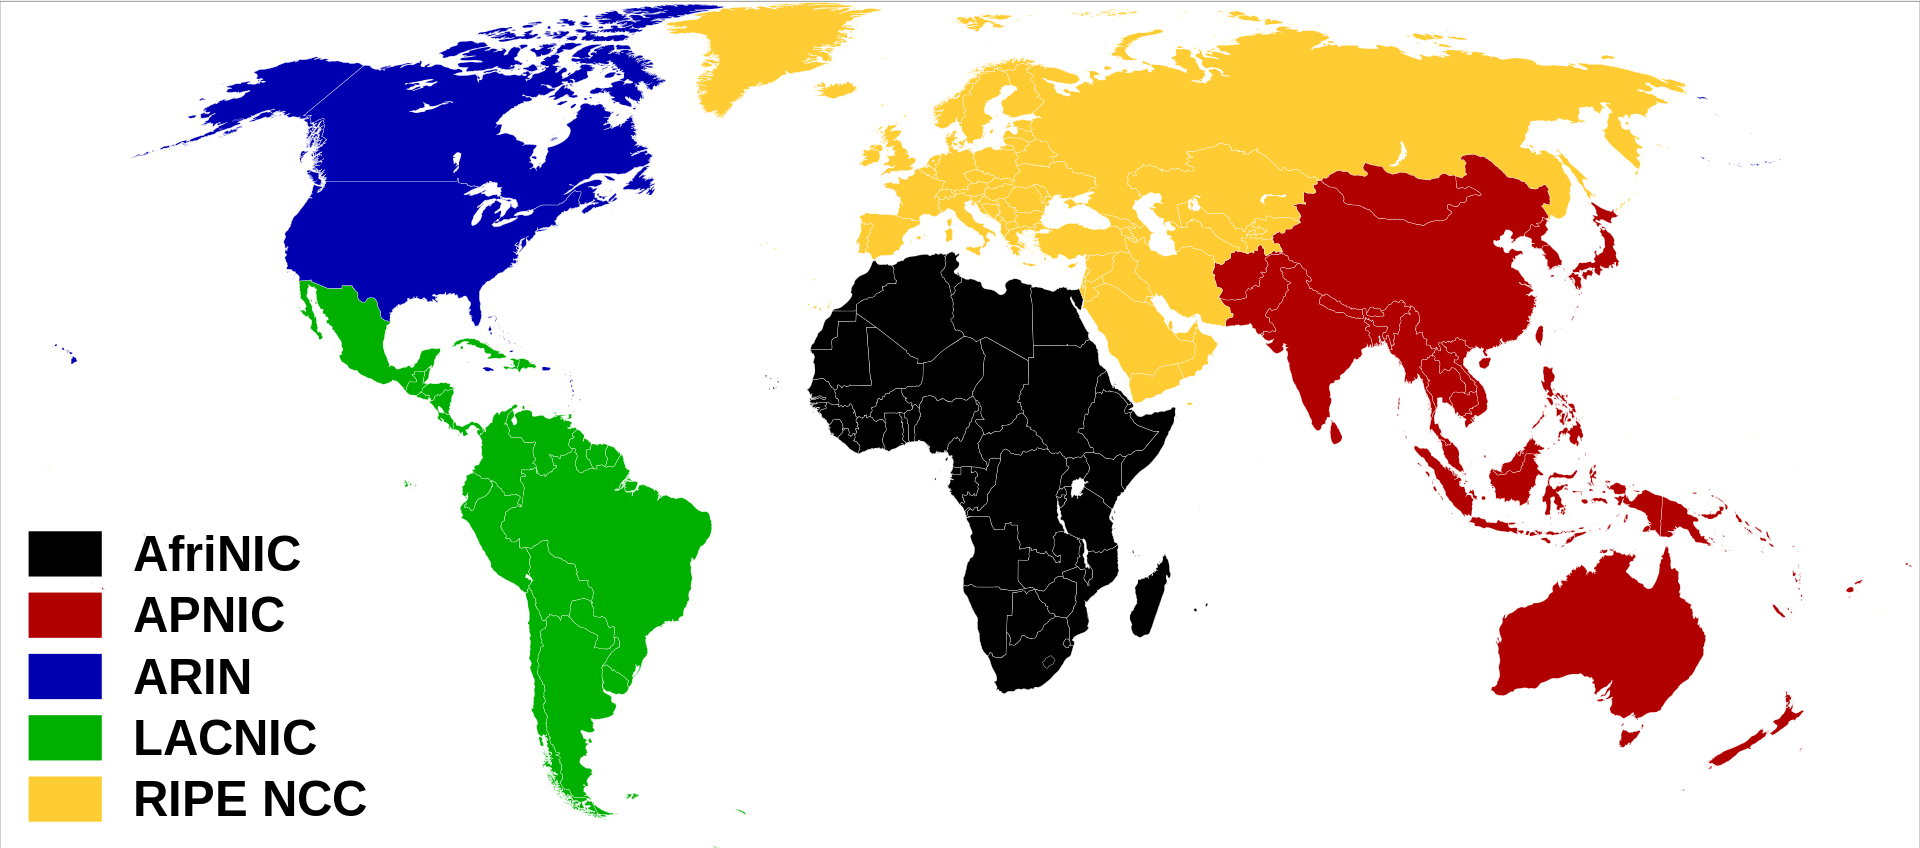
\includegraphics[width=\linewidth]{images/rirs.png}
  \caption{Regional Internet Registries manage the IP block assignment and Autonomous Systsem Number assignment for geographically local areas.}
  \label{fig:rirs}
\end{figure}

Before one can understand the weaknesses of Internet routing, one must understand how the Internet routing system is intended to work.  Individuals and organizations rely on Internet Service Providers (ISPs) to direct their network traffic to the appropriate destinations.  Any organization that wants to connect to the Internet must be given an IP address from an ISP or a block of IP addresses from a regional organization that manages IP address assignments known as a Regional Internet Registry (RIR).  Figure \ref{fig:rirs} shows examples of RIRs and the regions which they manage the IP space for.  Oragnizations that that want a set of their own IP addresses must also be assigned an Autonomous System Number (ASN).  ASNs are unique numbers which identify an organization's network in the global Internet.  It is common for a network to be assigned a single ASN and one or many contiguous blocks of IP addresses, as seen in Figure \ref{fig:rir-assignments}.

\begin{figure}
  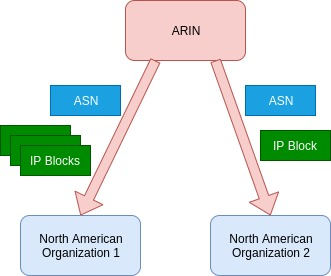
\includegraphics[width=\linewidth]{images/rir-assignments.jpg}
  \caption{Regional Internet Registries often assign a single ASN for each organization.  They also often assign one or many contiguous IP blocks to those organizations.}
  \label{fig:rir-assignments}
\end{figure}

\section{Internet Routing Operation}
In order to reach a service like Youtube, users need to know how to reach the service.  Youtube may have a set of IP addresses to allow users to connect to, but there are still two technical challenges:
\begin{enumerate}
 \item Youtube needs to announce where those IP addresses exist in the Internet
 \item The Internet itself needs to announce the path to take in order to get there to potential users
\end{enumerate}
The Border Gateway Protocol (BGP) is used to solve these problems, and its operations are illustrated in Figure \ref{fig:bgp-ops}.  The organization that owns the IP addresses announces those addresses as an IP prefix \footnote{An IP prefix could be one of the blocks assigned to the organization, or it could be a contiguous subset of IP addresses within that block.} into its upstream ISP, which takes care of challenge 1.  In that same announcement, Youtube also announces its ASN.  When Youtube's ISP connects to another network, it appends its own ASN to the list.  This process continues throughout the Internet, allowing for each network to know which path or paths it can take to reach Youtube.  These paths, known as AS paths, should all begin with Youtube's ASN, which effectively acts as a mapping between Youtube and the IP space in the global Internet.  These AS paths are used to address challenge 2.

If there are multiple paths to a target IP address, BGP uses a decision process similar to that in Figure \ref{fig:bgp-dec} \footnote{The BGP decision process is not standardized, and it may vary across different implementations.  Many implementations are very similar.}.  One of the most critical steps in the decision process, especially in the ISPs BGP decision making, is the AS path length.  It is often the case that the path with the shortest AS path length is the preferred route for traffic to a destination with a given IP address.

\begin{figure}
  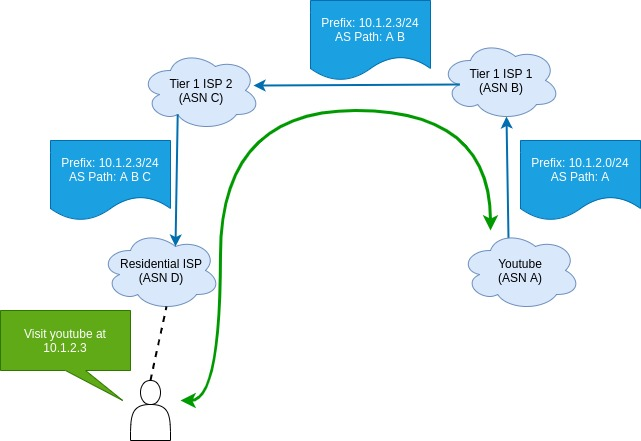
\includegraphics[width=\linewidth]{images/bgp-ops.jpg}
  \caption{The Border Gateway Protocol is used to announce the source of IP prefixes into the global Internet and to create paths from other organization's networks to those IP addresses.  The blue path represents the flow of BGP announcements for the Youtube IP prefix, and the green path represents the user's actual Youtube traffic.}
  \label{fig:bgp-ops}
\end{figure}

\section{BGP Hijacking}
With an understanding of how BGP operates, it is now useful to revisit the case of Youtube and the state run network of Pakistan.  What happened was Pakistan's state run network attempted to take all traffic destined for IP addresses in Youtube's IP prefixes and send them to a place in its own internal network that connected to nothing.  By mistake, this change in their internal network was announced, via BGP, to the rest of the world.  Figure {fig:bgp-hijack} illustrates what may have happened for some users who experienced a Youtube outage.  This problem is known as BGP Hijacking, and this example illustrates that the BGP has an inherent weakness: the receiver of the BGP announcement trusts the sender of the announcement, who in turn trusted the sender of the previous BGP announcement, and so on.  This trust model is known as "transitive trust", and it is part of why BGP scales well and part of why BGP is not secure.  BGP Hijacking can be unintentional, such as the Youtube example, but it can also be weaponized by others with malicious intent for data interception or denial of service.  It turns out that both intentional and unintentional BGP hijacking occur on a near-daily basis[1].  This is why it is so important that mitigation techniques be deployed across the Internet to avoid this weakness.

\begin{figure}
  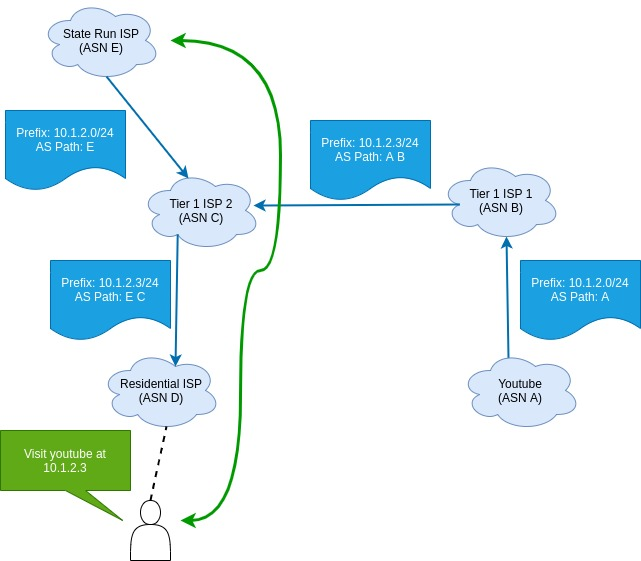
\includegraphics[width=\linewidth]{images/bgp-hijack.jpg}
  \caption{The state run network of Pakistan announced ownership of Youtube's IP prefixes to the rest of the world.  For many users, this ended up being the shortest AS path between them and Youtube.  The blue path represents the flow of BGP announcements for the Youtube IP prefix, and the green path represents the user's actual Youtube traffic.}
  \label{fig:bgp-hijack}
\end{figure}

\section{BGP Hijacking Mitigation Techniques}
There are various techniques which can me used to mitigate the weaknesses in BGP, each with varying effectiveness and cost.  Three techniques discussed below are Filtering, Resource Public Key Infrastructure (RPKI), and the BGPsec protocol.

\subsection{Filtering}
Filtering is a longstanding technique to both avoid accidental announcements as well as to prevent propagating incorrect announcements from neighbors.  There are a litany of BGP filtering methods, but two examples are AS path filtering and IP prefix filtering.  AS path filtering is a technique where only a set of whitelisted ASNs are allowed to be sent or accepted in BGP announcements.  This can particularly be effective at ISPs which directly interface with organizations, as those ISPs can choose to only accept AS paths comprised of the organization's ASN.  Organizations can similarly apply AS path filtering on egress of their announcements to avoid accidental propagation of incorrect ASNs.  IP prefix filtering is similar to AS path filtering, only it is applied to specific whitelisted IP prefixes.

The primary upsides of filtering approaches are that they are widely available and they are computationally inexpensive.  The downsides of filtering are that it is not a precise tool, and it can only be applied in certain cases.  Furthermore, it needs to be configured case-by-case\footnote{For example, an ISP serving thousands of organizations would need to configure filtering for ASNs and IP prefixes for each organization individually.  These values can change over time.}, making it rigid and difficult to maintain over time.  Finally, filtering methods cannot be applied in all cases.  They really need to be applied as close to the edge as possible, meaning the problems associated with transitive trust are still present.  Filtering methods have been around for a long time, and given that BGP hijacking events are still relatively frequent, it is clear that newer methods should be deployed to secure Internet routing.

\subsection{Resource Public Key Infrastructure for Origin Validation}
At this point, an astute reader may have observed that the RIRs have a central mapping of IP prefixes to ASNs, and the first ASN in an ASN path should correspond to the associated IP prefix in an announcement.  The question becomes, can this mapping of ASNs to IP prefixes be used to validate BGP announcements?  This approach is commonly used by operators who are manually trying to uncover BGP Hijacking events after they have occurred, but it is also the primary concept behind Resource Public Key Infrastructure (RPKI).  RPKI attempts to automate this approach by having a central authority (the RIRs in this case) host digitally signed information, known as Route Organization Authorizations (ROAs) confirming that an AS has the authority to announce a prefix.  Different RIRs implement this in different ways, but one example is presented in Figure \ref{fig:rpki-assignment}.  As shown in Figure \ref{fig:rpki-ops}, a BGP router can validate the origin of an announced prefix against the ROA database before it accepts the routes in the announcement.

The upsides of RPKI are that it provides explicit protection against the issue seen in the Youtube incident, and it can be added onto existing Internet routing infrastructure with minor changes.  The downside to RPKI is that it can be more computationally expensive\footnote{The cryptographic operations can be offloaded to a device which is attached to the router, which makes computational cost less of an issue} than standard BGP and it requires additional backend infrastructure which can result in more outages or misconfigurations, such as when a router is unable to obtain the latest ROAs to validate a new BGP announcement.

\begin{figure}
  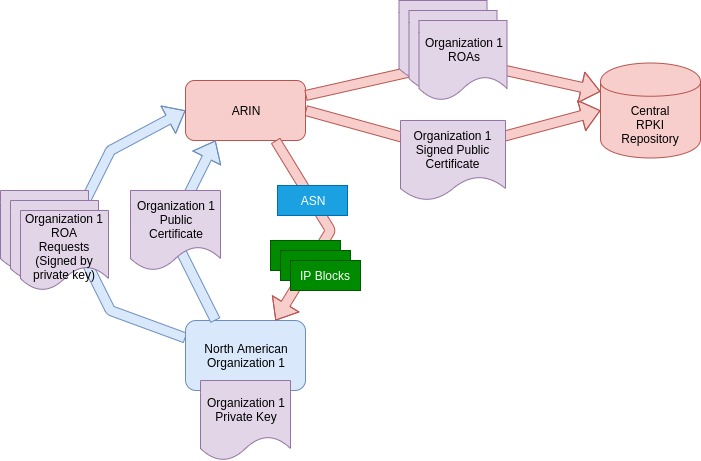
\includegraphics[width=\linewidth]{images/rir-rpki-assignments.jpg}
  \caption{This is an example of how ARIN implements RPKI.  The organization is assigned an ASN and a set of IP blocks.  If the organization participates in RPKI, then it generates a private key and a public certificate.  It sends the public certificate to be signed by the RIR.  The organization also generates ROA requests for its ASN and IP blocks, and it signs the request with its private key.  If ARIN deems the ROA request valid, then it generates an ROA and places it in the ROA database, where it can be used to validate the origin of BGP prefixes.}
  \label{fig:rpki-assignment}
\end{figure}

\begin{figure}
  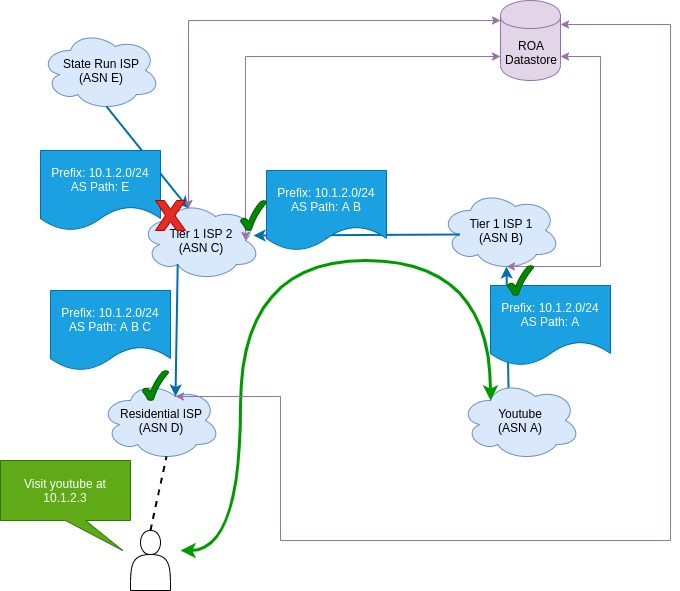
\includegraphics[width=\linewidth]{images/rpki-ops.jpg}
  \caption{If RPKI origin validation is in use, then routers can verify each BGP announcement by verifying that the first ASN in the AS path matches the origin of the IP prefix in the ROA database.  If there is a match, then the announcement is accepted and the associated routes may be propagated through the Internet.  If there is no match, then the route in the advertisement can be rejected.}
  \label{fig:rpki-ops}
\end{figure}

\subsection{BGPsec}
RPKI does a good job of preventing a lot of BGP Hijacking issues, but it turns out that it doesn't resolve all of them.  Go back to the case of malicious actors who want to intercept data.  RPKI will prevent them from claiming ownership of an IP prefix which they do not own, but it does not prevent them from announcing an AS path through their network to an IP prefix associated with its correct ASN as illustrated in Figure \ref{fig:bgp-intercept}.  Once traffic arrives in their network, they could either terminate it or passively spy on it.  A protocol known as BGPsec attempts to mitigate this issue by leaning on the RPKI infrastructure not only for prefix origin validation, but also for hop-by-hop AS path change validation.  BGPsec replaces the AS path with what it calls a BGPsec path, and it places extra requirements on how the path can be modified.  First, the AS performing modification can only provide its own ASN along with the ASN of the neighbor that the BGPsec announcment is being sent too.  Second, the AS originating the announcement must provide a signature creating using the organization's private key issued as part of RPKI which can validate that it added its ASN to the BGPsec path and that the announcement was intended for the recipient of the ASN.  BGPsec operations are showin in Figure \ref{fig:bgpsec-ops}.

The updsides of BGPsec are that it prevents all of the presented cases of BGP hijacking and it explicitly breaks the transitive trust property in BGP without losing the ability to scale.  The downsides are that it requires significantly more computation\footnote{The announcement construction and cryptographic operations in BGPsec need to be performed per neighbor per prefix, whereas with standard BGP an announcement can be created with no cryptographic functions and then sent with multiple prefixes to all neighbors} full replacement of the existing Internet routing protocol.  Also, while BGPsec does have an approach to allow for incremental adoption through interoperation with standard BGP, an advertisement where the full path is not secured through BGPsec is still susceptible to attack.


\begin{figure}
  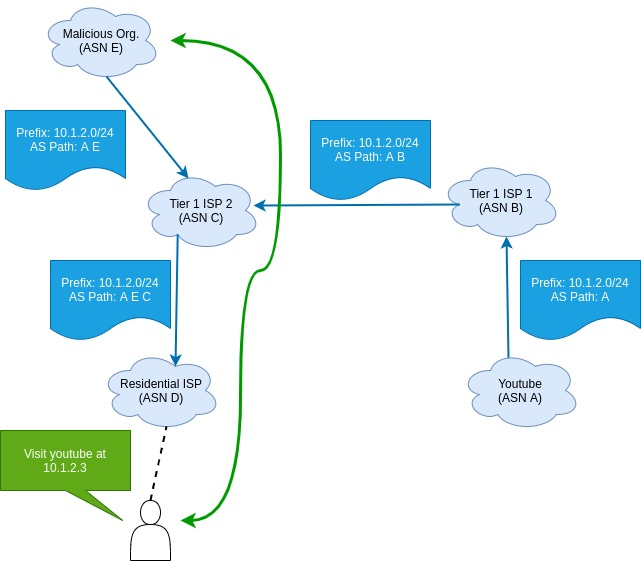
\includegraphics[width=\linewidth]{images/bgp-intercept.jpg}
  \caption{A malicious actor could announce a bogus route for a prefix with an AS path that includes the correct originating ASN and the malicious organization's ASN in the middle.  The malicious organization could choose to either terminate the connection by doing something like hosting a fake version of Youtube, or they could pass the traffic along to the real Youtube and capture the traffic passing through for offline analysis.  If this information includes encrypted financial information such as bank account numbers, then offline analysis could return highly valuable information.}
  \label{fig:bgp-intercept}
\end{figure}

\begin{figure}
  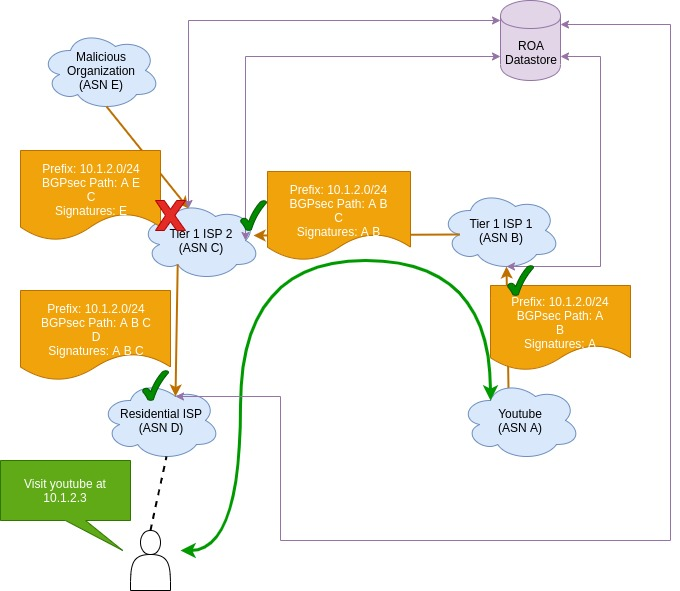
\includegraphics[width=\linewidth]{images/bgpsec-ops.jpg}
  \caption{If BGPsec is in use, then routers can verify each BGP announcement by verifying that each ASN in the BGPsec path has signatures which match the ROA database.  If each ASN in the path has valid signaturse, then the announcement is accepted and the associated routes may be propagated through the Internet.  If any single ASN in the path does not match, or if the origin ASN does not own the advertised prefix according to the ROA database, then the route in the advertisement can be rejected.}
  \label{fig:bgpsec-ops}
\end{figure}

\section{Conclusion}
This chapter illustrated the key weakness of transitive trust in the Internet routing protocol known as BGP, and it showed how this weakness can be exploited through BGP hijacking.  Multiple mitigation techniques for this weakness were introduced, including traditional approaches such filtering as well as newer approaches such as RPKI for origin validation and BGPsec.  BGP hijacking has been shown to occur on a near-daily basis, and thus the traditional filtering methods were shown to be insufficient to address the BGP hijacking problem at Internet scale.


[1] https://www.noction.com/blog/bgp-hijacking

\end{document}
